\documentclass[12pt]{article}

%% General
\usepackage{enumitem}
\usepackage{verbatim} 
\usepackage[utf8]{inputenc}

% URL
\usepackage{hyperref}

% Colour

\usepackage{xcolor}

\begin{comment}
%Header

\usepackage{fancyhdr}
\pagestyle{fancyplain}
\fancyhead{} % No page header - if you want one, create it in the same way as the footers below
\fancyfoot[L]{} % Empty left footer
\fancyfoot[C]{} % Empty center footer
\renewcommand{\headrulewidth}{0pt} % Remove header underlines
\renewcommand{\footrulewidth}{0pt} % Remove footer underlines
\setlength{\headheight}{0pt} % Customize the height of the header
\end{comment}


% Captions
\usepackage[margin=10pt,font=small,labelfont=bf, labelsep=endash]{caption}

%% Geometry

\usepackage[margin=1in]{geometry}


%% Maths

\usepackage[centertags]{amsmath}
\usepackage{amsfonts}
\usepackage{amssymb}
\usepackage{amsthm}
\usepackage{newlfont}

\theoremstyle{plain}
%\theoremstyle{margin}
{\swapnumbers
\newtheorem{thm}{Theorem}[section]
\newtheorem{cor}[thm]{Corollary}
\newtheorem{lem}[thm]{Lemma}
\newtheorem{prop}[thm]{Proposition}
}
%
\theoremstyle{definition}
%\newtheorem{defn}{Definition}[section]
%\newtheorem{nota}{Notation}[section]
%\theoremstyle{margin}
{\swapnumbers
\newtheorem{defn}[thm]{Definition}
\newtheorem{nota}[thm]{Notation}
\newtheorem{parag}[thm]{}
\newtheorem*{parstr}{\addtocounter{thm}{1}\thesection.\arabic{thm}*}
\newtheorem*{intropar}{\addtocounter{thm}{1}\arabic{thm}}
}
%
\theoremstyle{remark} {\swapnumbers
\newtheorem{rem}[thm]{Remark}
\newtheorem{exam}[thm]{Example}
\newtheorem{lemma}[thm]{Lemma}
\newtheorem{claim}[thm]{Claim}
}


%% Graphics
\usepackage{graphicx} 
\graphicspath{{Figures/}} 
\usepackage{subfig}

%% Tables
\usepackage{booktabs}
\usepackage{rotating}

% Allows shading of table cells
\usepackage{colortbl}

% Define a simple command to use at the start of a table row to make it have a shaded background
\newcommand{\gray}{\rowcolor[gray]{.9}}

%% Commands
\newcommand{\bd}{\textbf}
\newcommand{\itt}{\textit}
%
\newcommand{\al}{\alpha}
\newcommand{\be}{\beta}
\newcommand{\de}{\delta}
%
\newcommand{\To}{\longrightarrow}
\newcommand{\RE}{\operatorname{Re}}
\newcommand{\IM}{\operatorname{Im}}
%
\newcommand{\QQ}{\mathbb{Q}}     
\newcommand{\RR}{\mathbb{R}}      
\newcommand{\ZZ}{\mathbb{Z}}      
\newcommand{\CC}{\mathbb{C}}      

\numberwithin{equation}{section}

%% Title

\begin{comment}
\setlength{\droptitle}{-8em} 
\title{	
\normalfont \normalsize \bf
\vspace{-1 em}} 
\end{comment}

%% Referencing

\usepackage[style=nature]{biblatex}

\usepackage{float}
\graphicspath{ {images/} }
%
\addbibresource{bib.bib}
%
\begin{document}

\title{Architecture of a Nucleus:\\Nuclear Spectra and Random Matrix Theory}
\author{Alexander Illarionov}
\date{July 18, 2015}
\maketitle
%
\section*{Introduction}

What is the structure of matter? From the philosophical concept of \itt{a tomos}, or an \itt{indivisible} discrete unit of matter, proposed by Leucippus and Democritus in the Vth century BC \cite{ato}, to the idea of many-body systems of subatomic particles, the answer to one of the oldest questions in the history of science evolves continuously. Modern understanding of an atom as a system of a nucleus surrounded by a smeared electron cloud rests on quantum theory, which fruitful edifice resulted from the theoretical and experimental efforts in the beginning of the XXth century. Despite the nomenclature, an atom \itt{is} divisible, as well as a nucleus and electrons are under certain conditions.\footnote{Isolated electrons \itt{are} indivisible, which accounts for the classification of an electron as an elementary particle. However, in 1982 the prediction was made that electrons in a one-dimensional chain of atoms could be split into three \itt{quasiparticles} with characteristic properties of an electron; a \itt{holon} carries the charge, a \itt{spinon} bears the spin, while an \itt{orbiton} takes the orbital location of the corresponding electron.\cite{kugel} The quasiparticles can move with different speeds and in different directions inside the material.\cite{merali} In 1996 separation of an electron into a holon and spinon was observed.\cite{kim} In 2012 splitting of an electron into an orbitron and spinon was detected.\cite{spin} The next milestone is to obtain empirical evidence for the simultaneous co-existence of all three quasiparticles.}

One of the major conundrums in atomic modelling is the fact that the electrons \itt{interact} with each other by exerting long-range Coloumb repulsion. All physical models, including models of interacting particles, are designed to describe fully the phenomena under consideration, like the motion of electrons in the atom or protons and neutrons in the nucleus. Nevertheless, there is no exact solution to the general problem of \itt{n} interacting bodies.\cite{nbody} The analysis of many-body systems like complex atoms and atomic nuclei is thus purposed to yield an approximating model matching experimental results.

In some cases the interaction of a single particle with all the others can be approximated by an average central field to a significant level of precision.\cite{shth} In case of an atom, the superposition of electric fields produced by the nucleus and electrons can be estimated by a suitable central potential averaged over time, identical for all electrons in the atom and varying as a function of the nuclear charge and distance from the nucleus.\cite{dem} If such a potential is found, the interaction not included in the average field, such as the interaction of electrons in the outer shell, should still be taken into account, which is usually achieved by treating this \itt{residual} interaction as a perturbation.\cite{shth} Hence any electron is viewed as independent of all the others, and the many-body problem is reduced to the well-defined problem of a one-electron motion. The description of a physical system consisting of interacting particles in terms of independent particles in an average central field is called a \bd{shell model}.\cite{shth} While shell theory successfully predicts the properties of electrons in an atom, the same tools which are used for the atomic shell model are not completely applicable to any nucleus due to inherent differences between the atomic and nuclear architecture:
\begin{enumerate}
\item The nuclear residual interaction is \itt{essentially} attractive. Although protons do repel each other, short-range strong nuclear force between the nucleons overcomes the effects of the long-range Coulomb interaction.
\item There is no \itt{apparent} reference point around which motion of nucleons occurs, which is present in an atom. The atomic reference point is a nucleus itself, in which the greatest part of the atomic mass is concentrated and in which potential electrons move. 
\item The energy values characteristic of nuclei are of the order of 1 MeV, or $1.602\times10^{-13}$ J. The energy values characteristic of atoms are of the order of 1 eV. Thus, excitation of an electrons is approximately a million times less energetically \itt{expensive} than that of a nucleus due to the strong interaction between the nucleons exceeding the effect of the Coulomb force holding electrons, which accounts for the importance of atoms in formation of matter and chemical reactions in general.
\end{enumerate}

Understanding of the nuclear architecture is crucial to understanding of the chemical diversity in the Universe. For instance, if the carbon-12 excited state at 7.65 MeV were nonexistent, not enough carbon would have formed for the reader to be amazed by the marvels of life.\cite{bur57}Although a substantial knowledge of forces governing the structure of a nucleus is available, there is no \itt{complete} nuclear theory \itt{explaining} the nuclear properties, including the properties of heavy and excited nuclei, in terms of the properties of the interactions between neutrons and protons.\cites{unif}{eis85} The complexity of a \itt{nontrivial} nucleus is not reflected fully by the proposed models. Nevertheless, the intricacies of the structure can tell us more than it may first seem. How can the \itt{statistical facade} characterise the architecture of a nucleus, and do prime numbers have the same distribution as nuclear energy levels?
\section*{Exciting Story of Nuclei}

What happens with a nucleus when it is hit by another nucleus or particle? In 1919 Rutherford experimentally showed that artificial nuclear transmutation was possible as a result of the collision between nitrogen nuclei and alpha particles.\cite{ruth19} In 1932, after irradiation of beryllium and boron with alpha particles Chadwick witnessed emission of a neutron.\cite{ch32} Do nuclear collisions always result in radiation or discharge of a particle? Can nuclear collisions be inelastic, with kinetic energy absorbed by the nucleus and distributed among the nucleons? And if inelastic nuclear collisions do take place, what would happen with such a nucleus in the long run?

The answers to these questions can be found by studying reactions of nuclei with protons and neutrons. Collisions between positively charged protons and nuclei are obstructed by the mutual Coulomb repulsion; the obstructing interaction is called the \itt{Coulomb barrier}. No such barrier exists in the nuclear reactions with neutrons. The Coulomb barrier is responsible for the possibility of elastic collisions between a nucleus and a proton; up to a particular energy value the kinetic energy of the proton is shared with the nucleus, which closely matches the notion of a point mass. When the Coulomb barrier is overcome, protons interact with a nucleus similarly to neutrons. 

Nuclear reactions can be divided into two categories: fast and slow. \cite{mehta} In fast nuclear reactions nucleons with high kinetic energy are absorbed; the reaction time is on the order of the time interval required for the incoming nucleon to pass through the region of space having the same size as the nucleus. The de Broglie wavelength of the nucleon is short, so it interacts with only a small fraction of nucleons inside the nucleus. In a typical direct collision another nucleon is emitted with the almost identical momentum, thus the correlation between the initial and final states of the system is strong. Slow nuclear reactions last approximately two or three times longer. The incident nucleon is quickly trapped and its energy and momentum are disseminated between the other nucleons before enough energy is centred on another particle to be ejected or for the nucleus to irradiate. In both fast and slow reactions the absorption of the incident nucleon depends on its kinetic energy; the probability that nuclear reaction takes place if the transferred energy matches specific values. Therefore, nuclear spectra are discrete, and energy levels of both atoms and atomic nuclei are quantised.

The process of neutron capture, when an incoming neutron is absorbed by a targeted nucleus, became important in the development of nuclear reactors from 1930s to 1970s, in the Golden Age of nuclear physics .\cite{firk} By studying the energies of excited nuclei obtained in the progress of slow nuclear reactions, Bohr argued that nuclear collisions with a slow neutron result in the formation of a relatively stable \itt{compound nucleus}.\cite{bo36} The compound state persists for a sufficient amount of time to \itt{lose all memory} of the way in which it was formed, and the subsequent decay is thus entirely independent of the initial conditions of the system. A wooden toy model in Fig \ref{fig:1} on page \pageref{fig:1} demonstrates Bohr's idea; nucleons are represented by billiards, kinetic energy of the incident neutron by a queue, and the trough simulates the mean attractive field of the nuclear interactions. Bohr's compound nucleus hypothesis was confirmed experimentally in the 1950s and 1960s by radiochemical analysis of radioactive nuclides produced using the same compound nucleus formed in different ways.\cite{hand}

\begin{figure}
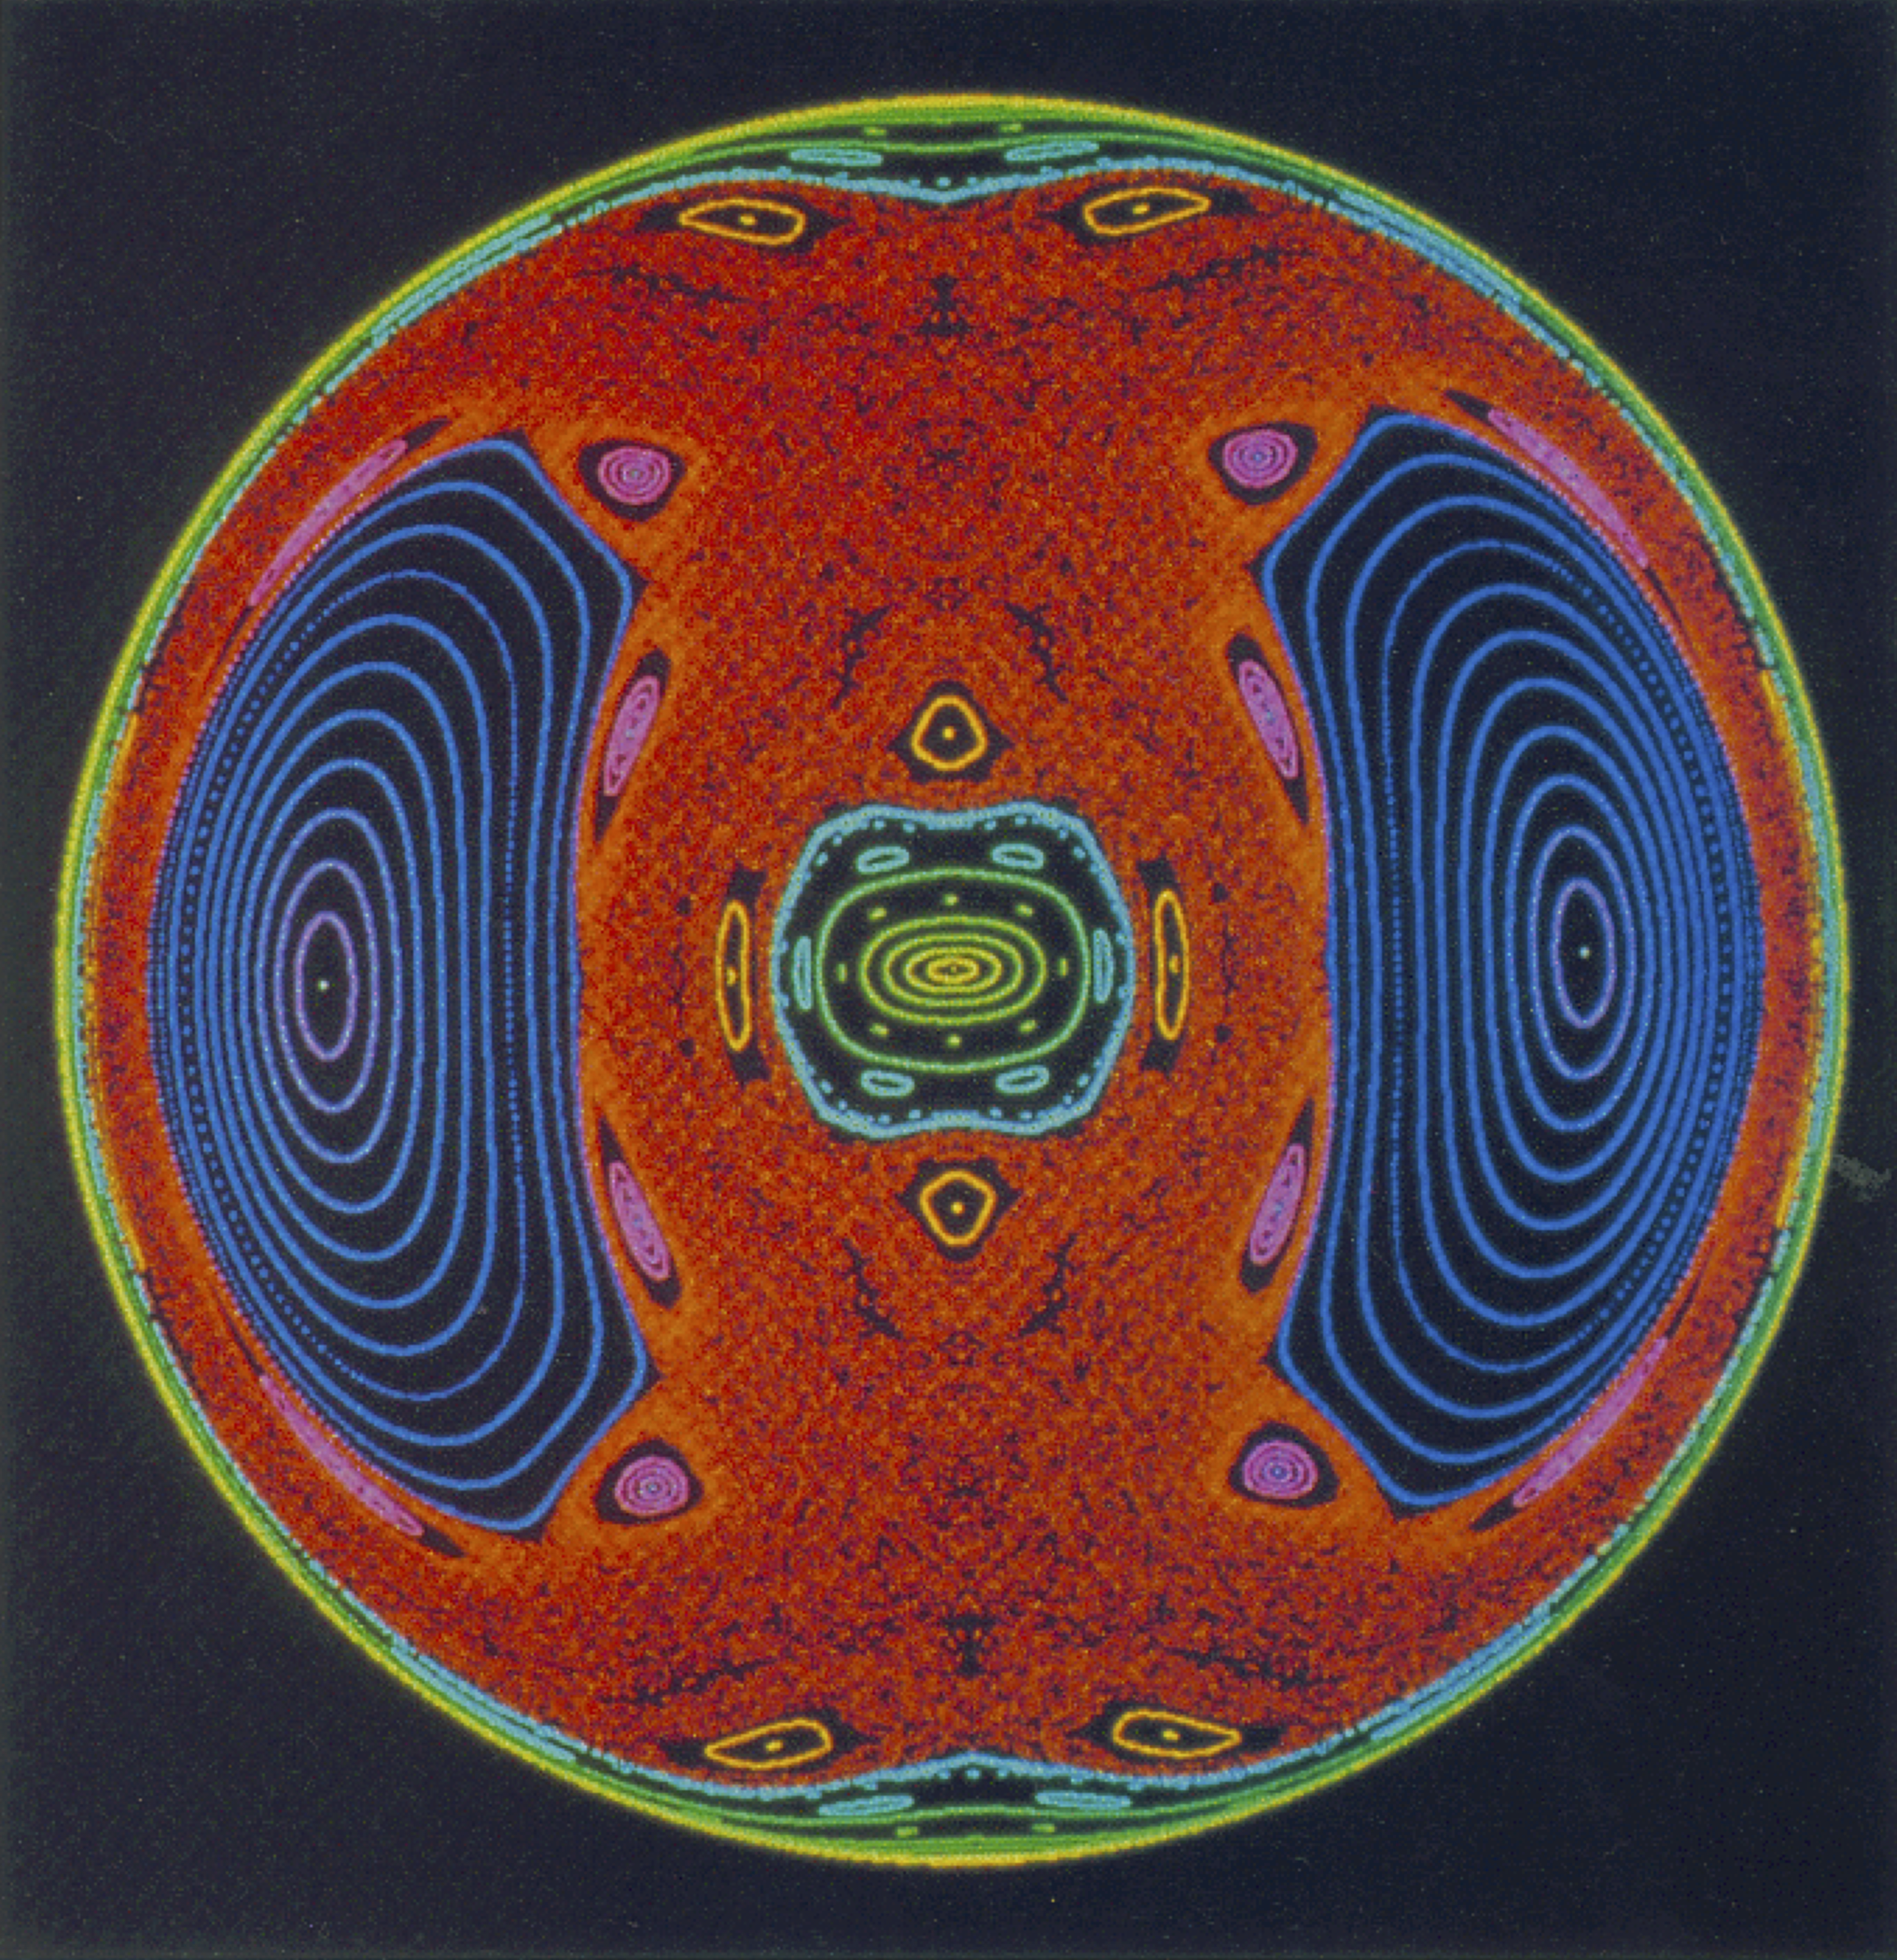
\includegraphics[width=\textwidth]{1}
\caption{Bohr's toy model shows graphically the compound nucleus hypothesis. Credit:\cite{bo36}}
\label{fig:1}
\end{figure}

The central phenomenological description of the nuclear structure is the shell model. The most important empirical evidence for the model is the existence of so-called \itt{magic} numbers. The electron configuration of noble gas elements is the most stable in the periodic table due to the fact that all the electron shells are closed and hence they possess "magic" atomic numbers 2, 10, 18, 36, 54, 86. Similar shell effects are present in the nuclei, and if either atomic or neutron number is one of the magic numbers 2, 8, 20, 28, 50, 82, then the nuclei are distinctly stable.\cite{hand} The reason \itt{why} the magic numbers was not clear until the independent work of Mayer\cite{mayer} and the group of Haxel, Jensen and Suess\cite{haxel}. The state of a single nucleon was considered in the averaged spherical field of all the other nucleons. The particles fill the nuclear energy levels according to the quantum numbers which also determine the maximum number of nucleons present in a single shell. When certain states are completed, a huge gap in the energy level diagram is observed. By taking into account strong correlation between spin and orbital angular momentum, the model reproduces the magic numbers.\cite{hand}

The energy levels of the ground state and low-lying excited state of various nuclei can also be predicted by the independent-particle shell model.\cite{mayer55} However, as the energy of the excited state increases, the relative error of the predicted values increases too with more and more nucleons being knocked out of the main body of the nucleus. At sufficiently high energies the energy levels overlap and mix so that it is impossible to explain single nuclear states without referencing to the others. When the intermixing is dominant, the individual characteristics of the nuclear energy levels can be successfully described by the average, statistical properties. \cite{mehta}

In the 1950s a new tool was devised which would not only change the field of nuclear physics but also have an extensive impact on such diverse fields as classical and quantum dynamics\cites{berry358}{gut}, number theory, complex analysis\cite{cart} and neuroscience\cite{wain13}.  The mathematical apparatus which provided an opportunity to study the universal properties of nuclear reactions came about as a result of the following facts\cite{firk}:
\begin{enumerate}
\item Neutrons accelerated to several electron-volts collide with nuclei to form compound nuclei excited to typical neutron binding energies, ranging from 5 to 10 million electron-volts.
\item Formation and decay of a compound nucleus is a statistical process of great complexity.
\item The advancement of experimental techniques, such as neutron time-of-flight method\cite{firk79}, allowed measurements of energies of compound nuclei with resolutions up to several keV.
\end{enumerate}
In the 1950s Professor Wigner introduced his surmise on the distribution of adjacent neutron resonances of the same spin and parity, which is an indicator how the nuclear structure looks like when the spatial coordinates of all the nucleons are reversed in sign. With Bohr's hypothesis, which essence is the strong interactions between the nucleons in the slow nuclear reaction, Wigner's surmise states that the generic characteristics of complex systems can be represented by the attributes of an \itt{ensemble}, or group, of random matrices with no system-specific properties but for the symmetries.\cite{wig67} The prolific field of Random Matrix Theory (RMT) was born.
\section*{Universal Randomness}
The physical system of a nucleus is described quantum mechanically.\cite{mehta} The energy levels of the system are nothing else but the eigenvalues $E_i$ of a \itt{Hermitian operator} $H$, or the \itt{Hamiltonian}\footnote{A Hamiltonian describes position and momentum of each member of the system}. In general, there is an infinite number of energy levels in a physical system. Since the Hamiltonian describes the energy levels of a system, it should operate in an infinite-dimensional space. Working with the infinite dimensions is difficult, therefore approximations are made, amounting to a truncation of the Hamiltonian which keeps only the parts relevant to our study. In the study of nuclear reactions, our interest lies in the discrete energy levels, and hence the operator in the infinite-dimensional space is reduced to a large but finite number of dimensions. The resulting Hamiltonians are then represented by finite matrices. If we can solve the Shr\"{o}dinger equation for the $i$th parts of the system:
\begin{equation*}
H\Psi_i=E_i\Psi_i,
\end{equation*}
all the energy values and corresponding wavefunctions will be determined. However, the problem with the nucleus is that the Hamiltonian is not known. Even if it \itt{were} known, finding the solutions to the Shr\"{o}dinger equations obtained is beyond the modern computational capability! Is there another way to describe nuclei meaningfully and predict their behaviour?

Since any particular information other than general properties of the system is not known, we are bound to make statistical hypotheses about the Hamiltonian. As F.Dyson puts it, "the statistical theory will not predict the detailed sequence of levels in anyone nucleus, but it will describe the general appearance and the degree of irregularity of the level structure that is expected to occur in any nucleus which is too complicated to be understood in detail."\cite{dy62}  The expectation is that by considering an ensemble of Hamiltonians formed according to the unknown, random rules which have physical meaning an ensemble average would describe to a significant level of precision the completely unknown system under consideration, since not many systems would differ drastically from the appropriately chosen Hamiltonian average. The expectation is \itt{not} that the ensemble average accurately or precisely describes specifically, for instance, $^{239}$U, and if it disagrees considerably, the properties not taken into account by the average Hamiltonian could be investigated. But how can the appropriate Hamiltonian ensemble be constructed in the first place?

There are three main considerations affecting the form of the ensemble\cite{mezz}:
\begin{itemize}
\item spacetime symmetries
\item isotropy in space
\item statistical independence of elements in the random matrix
\end{itemize}
The first and second conditions are physical. Is the physical system time-reversal invariant? What is the parity of the system? Is any direction of space \itt{preferred}? The third factor is the requirement of mathematical simplicity, which is not necessary in the description of the system but which reduces the complexity of mathematical operations involved. 

Nuclei are time-reversal invariant.\cite{rmc7}  For physical systems with such a symmetry their Hamiltonians are \itt{symmetric} and have real elements. These properties ensure that the aforementioned approximation of nuclear Hamiltonians \itt{is} manageable. The other spacetime symmetries which determine the ensemble are parity and rotational symmetry. The ensemble is constructed with symmetries of the Hamiltonians taken into account; only real and symmetric $N\times N$ matrices are included. To ensure the isotropy, the ensemble is invariant under transformations which leave the Hamiltonians invariant. The elements of the matrices are defined randomly by a distribution of choice. In fact, the density and the spacing distribution, which indicates how the differences between the energy levels behave, are independent of the many characteristics of the chosen distribution.\cite{rmc7} The ensemble of random matrices constructed by the mentioned procedure is called Gaussian Orthogonal Ensemble(GOE). It is worth mentioning that Wigner's surmise, which is based on simple heuristical reasoning, matches closely the nearest neighbour spacing distribution given by GOE(cf. Fig \ref{fig:2}). 

\begin{figure}[H]
\includegraphics[width=0.5\textwidth]{2}
\centering
\caption{The probability density versus the scaled spacing given by GOE(p(0,s)) and Wigner's surmise(p$_w$(s)). Credit:\cite{ga61}}
\label{fig:2}
\end{figure}

There are several statistical observations which prompt the application of RMT to the study of the nuclear structure and reactions\cite{mehta}:
\begin{enumerate}
\item The greater the excitation energy, on average the smaller the difference between the consecutive energy levels; thus, the level density increases as the excitation energy grows. Nevertheless, energy levels in the discrete region do not get arbitrarily close.Moreover, although level densities in different nuclei may not coincide, the fluctuations, or the divergence from the mean density, in the precise energy levels do not seem to be characteristic of the nucleus or depend on the excitation energy. This property is called \itt{spectral rigidity}.
\item It seems that nuclear energy levels with different spin and parity do not affect the position of each other. However, energy levels with equal quantum numbers exhibit apparent regularity; for instance, so-called \itt{level repulsion} is observed, since the energy levels are rarely positioned close to each other.
\item Due to the variety of the differences between the nuclear energy levels, the excited nuclei may either eject a neutron or a quantum of radiation. The statistic of \itt{reduced neutron width}, which allows unambiguous comparison of the decay energy, varies considerably from level to level. 
\end{enumerate}

How can the predictions of RMT be tested on the experimental values of nuclear spectra? For the statistical hypothesis testing to be meaningful, several criteria are implemented in choosing the data. The requirements are the following\cite{gom11}: 
\begin{enumerate}
\item The sequence of the nuclear resonances should be as long as possible.
\item The quantum numbers of the nuclear resonances under consideration should be accurately known and be identical.
\item The sequence should be complete with no missing energy levels.
\end{enumerate}
These conditions are experimentally difficult to satisfy; despite more than 60 years of intense work on the problem of nuclear spectra, the appropriate data is still scarce.\cite{wei14}

The graph comparing the spacing of  108 $^{166}$Er nuclear resonances and the GOE prediction is given in Fig \ref{fig:3}. Distinctness of the data from the Poisson prediction is clearly visible.
\begin{figure}[H]
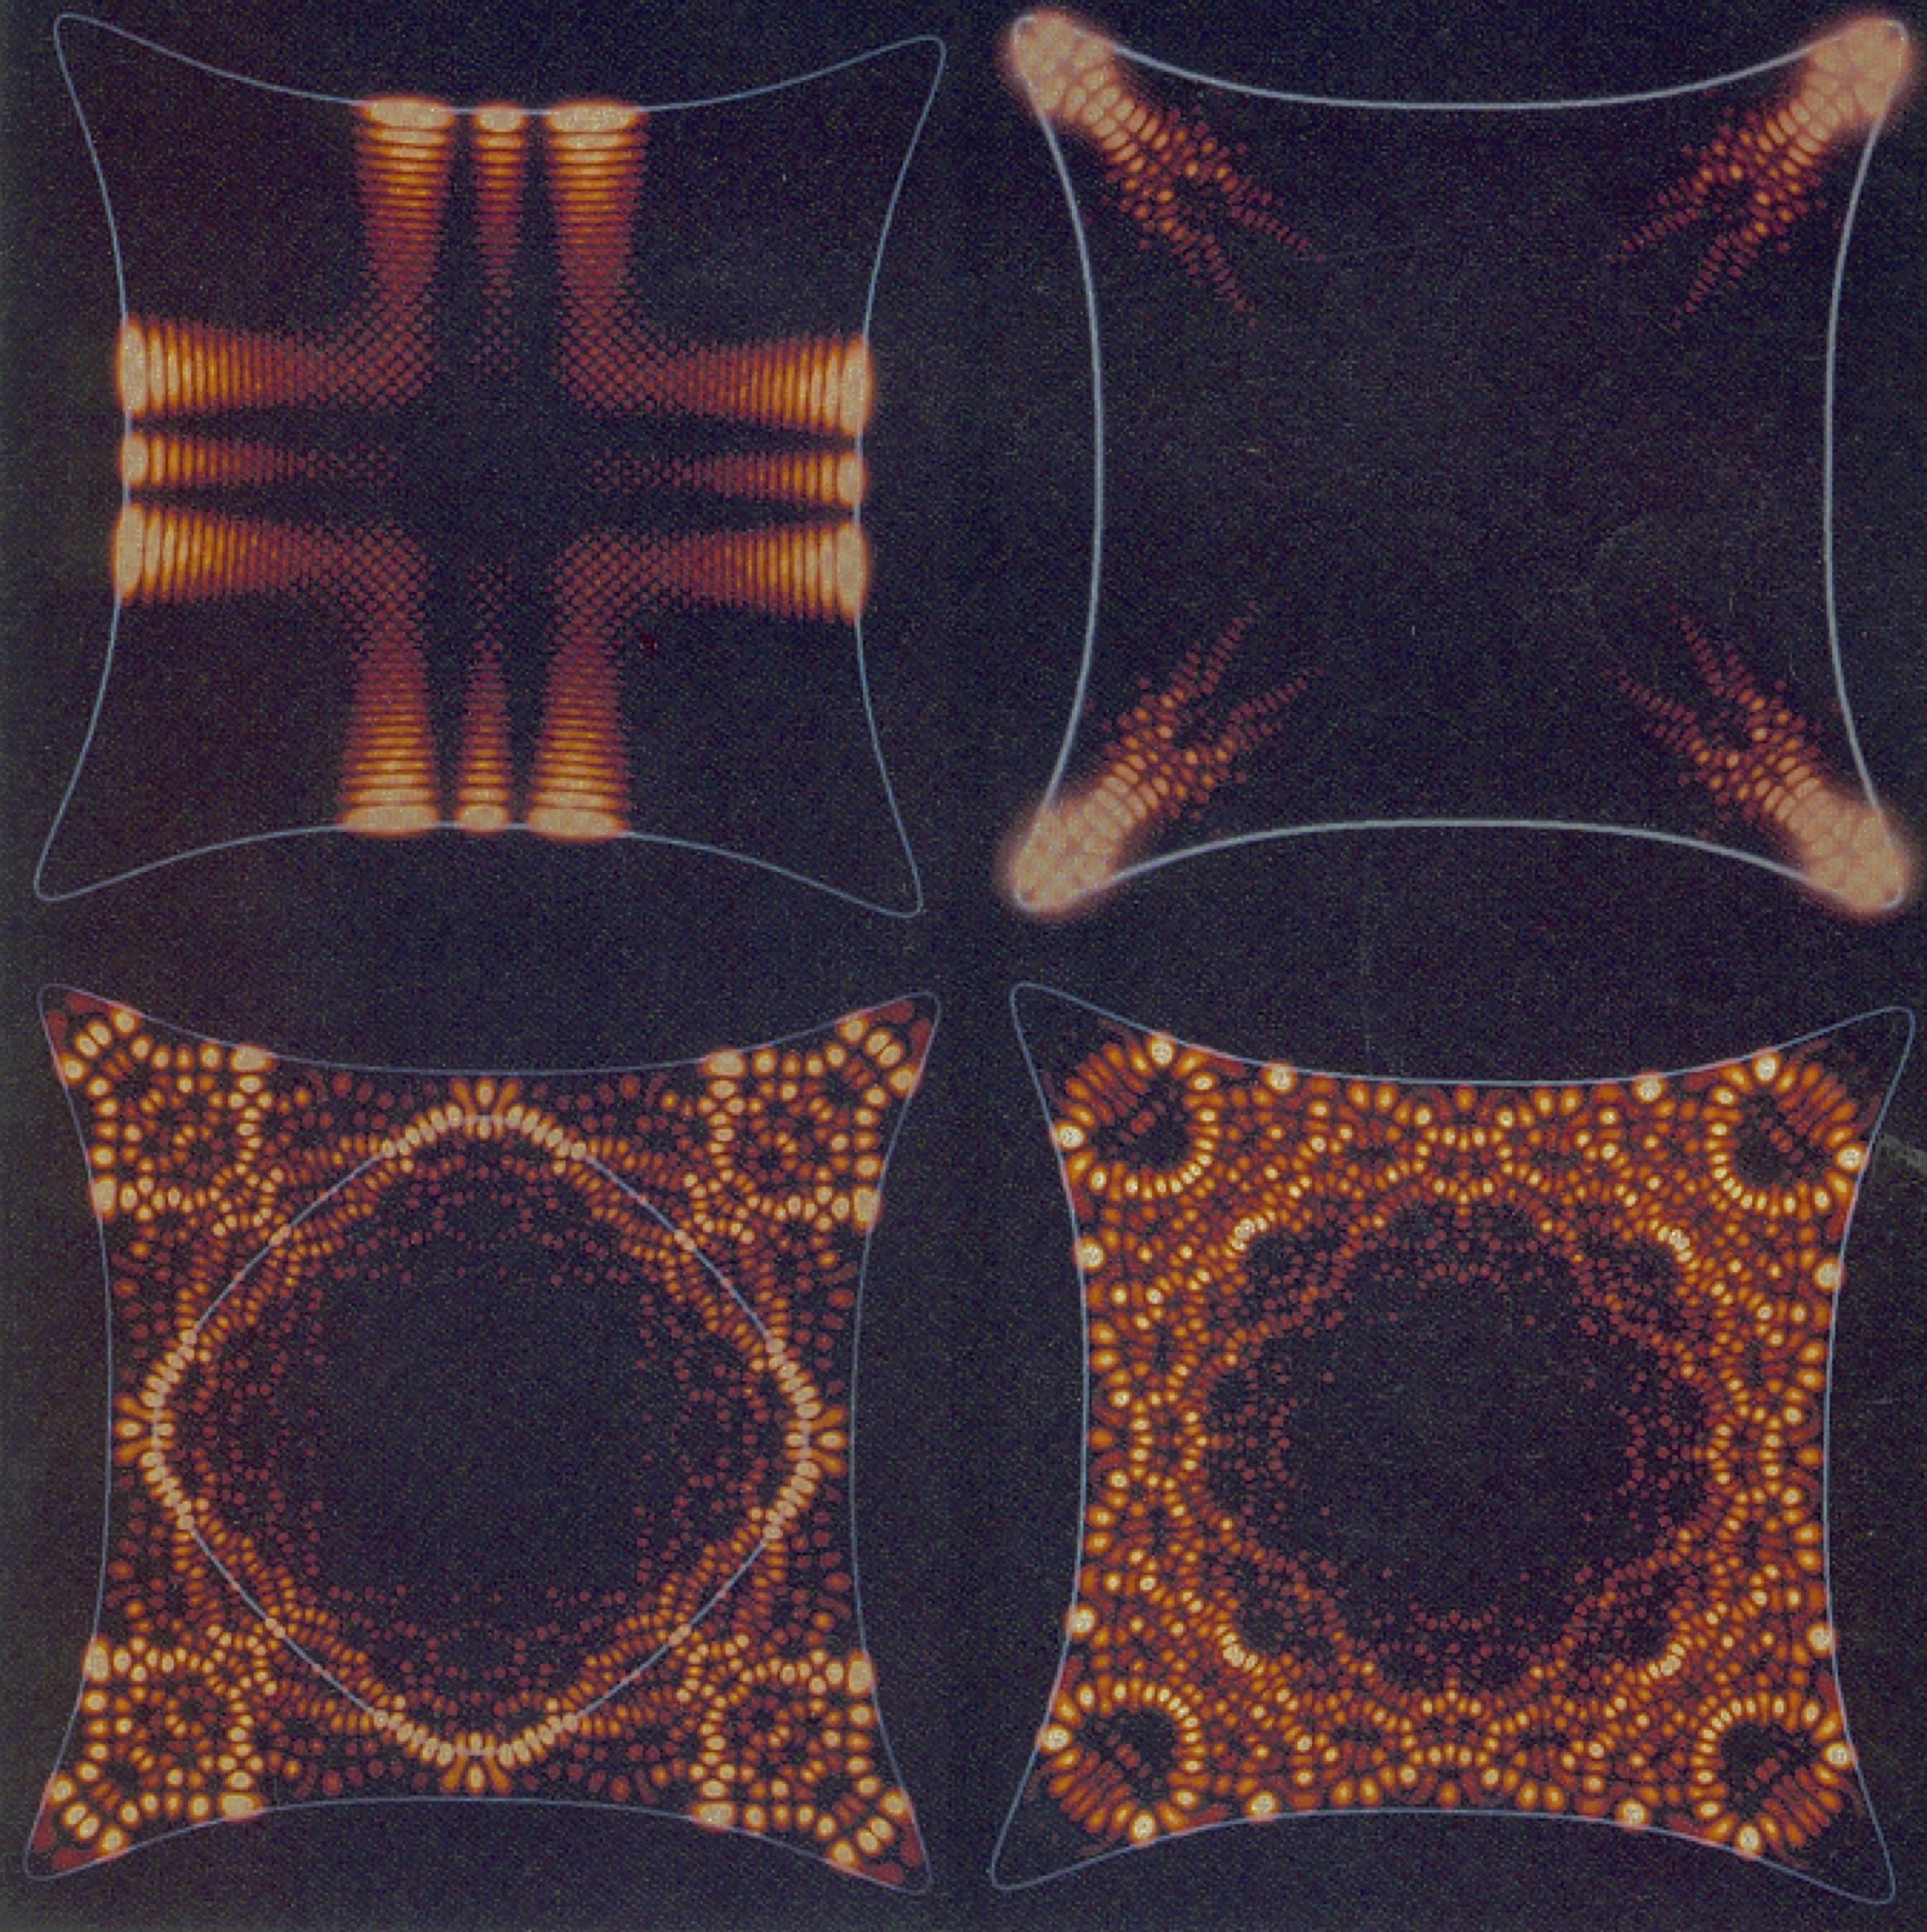
\includegraphics[width=0.5\textwidth]{3}
\centering
\caption{Nearest neighbour spacing of 108 $^{166}$Er nuclear resonances. The solid curve showing the Poisson distribution indicates the spacing distribution of entirely uncorrelated sequence. Credit:\cite{ga61}}
\label{fig:3}
\end{figure}

The different approach to the problem, developed by Bohigas, Haq and Pandey\cite{ga61} in 1983, was to introduce two novel ingredients to the traditional analysis of the nuclear resonances(for the historical perspective see \cite{mezz}): 
\begin{enumerate}
\item Instead of the sequence comparison of individual nuclei, a group of nuclei with the same quantum numbers were included in the relatively expansive Nuclear Data Ensemble(NDE) with information on a total of 1407 nuclear resonances.
\item A new method of statistical hypothesis testing was devised.
\end{enumerate}
The result is given in Fig \ref{fig:4}.
\begin{figure}[H]
\includegraphics[width=0.5\textwidth]{4}
\centering
\caption{Level spacing histogram for the NDE. Credit:\cite{ga61}}
\label{fig:4}
\end{figure}
The NDE or its modifications which include recently obtained data form the basis of modern work on the level-spacing distribution.\cite{wei14} Further statistical testing yielded strong support for the agreement of the empirical evidence with the predictions of Random Matrix Theory.\cite{lom94}  Not only nuclear resonances seem to be unfolded by RMT, but also the key to the distribution of the number-theoretical building blocks seems to lie in the universal properties of random matrices: prime numbers.
\section*{Spectra of Primes}
Consider the following function $\zeta:\CC\to\CC$ defined for $s\in\CC$ such that $\Re \left({s}\right) > 1$:
\begin{equation*}
\zeta \left({s}\right) := \sum_{n \mathop = 1}^\infty n^{-s}
\end{equation*}
The error term of the formula giving an approximation to the prime-counting function, which outputs the number of primes less than or equal to some real number, depends on the zeros of this function, called the \itt{Riemann zeta function}. The definition of the Riemann zeta function can be extended to run over all $s, s\neq1$.\cite{riemann} The \itt{trivial zeros}, -2, -4, -6, -8, etc. are known from such an extension. Nevertheless, for the nontrivial zeros it is only known that all of them are contained in the \itt{critical strip} $0<\Re\left({s}\right)<1$. The celebrated Riemann Hypothesis states that all nontrivial zeros lie on the \itt{critical line}  $\Re(\left{s}\right)=\frac{1}{2}$. There is no counterexample to the conjecture for the first 10 trillion zeros.\cite{gou}

In the 1970s Montgomery and Dyson noticed the connection between the pair correlation of the $\zeta \left({s}\right)$ zeros and the correlation of the eigenvalues of complex Hermitian matrices, which possess the symmetry of \itt{self-adjointness}.\cite{mont} In RMT, the ensemble of random Hermitian matrices is called Gaussian Unitary Ensemble(GUE). With the advancement of computing technologies and algorithms, the mathematician Andrew M. Odlyzko embarked on the calculation of the zeros high above the critical line.\cites{od87}{od01} The Montgomery-Dyson conjecture astoundingly fitted the data of Odlyzko(cf. Fig \ref{fig:5}, \ref{fig:6}, \ref{fig:7}).
\begin{figure}[H]
\includegraphics[width=0.5\textwidth]{5}
\centering
\caption{Pair correlation function for the zeros $\frac{1}{2}\pm i\gamma_n$, where $\gamma_n\in\RR$, of the Riemann zeta function for $1<n<10^5$. The solid curve indicates the Montgomery-Dyson conjecture. Credit:\cite{od87}}
\label{fig:5}
\end{figure}
\begin{figure}[H]
\includegraphics[width=0.5\textwidth]{6}
\centering
\caption{$10^12<n<10^12+10^5$. Credit:\cite{od87}}
\label{fig:6}
\end{figure}
\begin{figure}[H]
\includegraphics[width=0.5\textwidth]{7}
\centering
\caption{Pair correlation function for 79 million zeros plotted around n$\approx10^{20}$. Credit:\cite{od01}}
\label{fig:7}
\end{figure}

Thus, RMT successfully predicts the statistical behaviour of the zeros of one of the most important functions in the history of mathematics.
\section*{Conclusion}
Random matrix theory provides an important tool in the study of various topics in mathematics, science and beyond. The behaviour of nuclear energy levels studied in light of RMT hints at the important properties of nuclei and processes behind nuclear reactions. 

RMT is not supposed to give precise description of physical phenomena. By definition, it lacks any variables in telling us the story of excited nuclei. Therefore, if there is a discrepancy in the prediction, RMT gives us a tentative test of the mechanisms other than symmetries which affect the evolution of the physical system. And the discrepancies \itt{do} exist.The main problem, however, lies in the experimental data conforming the stringent conditions required for the significant statistical testing. Such data is scarce, but new details emerge continuously. Stay tuned.
\printbibliography
%
\end{document}